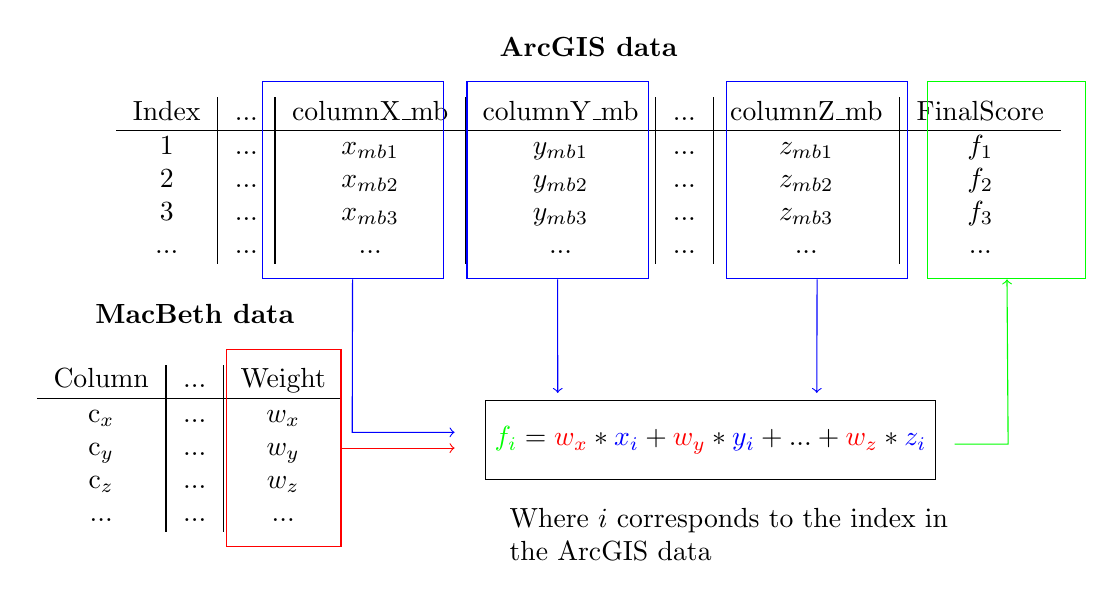
\begin{tikzpicture}
    % Tables
    \node (tab1) {%
        \begin{tabular}{c|c|c|c|c|c|c}
            Index  & ... & columnX\_mb & columnY\_mb & ... & columnZ\_mb & FinalScore \\
            \hline
            1 & ... & $x_{mb1}$ & $y_{mb1}$ &... & $z_{mb1}$ & $f_{1}$ \\
            2 & ... & $x_{mb2}$ & $y_{mb2}$ &... & $z_{mb2}$ & $f_{2}$ \\
            3 & ... & $x_{mb3}$ & $y_{mb3}$ &... & $z_{mb3}$ & $f_{3}$ \\
            ... & ... & ... & ... & ... & ... & ...
        \end{tabular}
    };
    \node [left,xshift=-3cm,yshift=-3.4cm] (tab2) {%
        \begin{tabular}{c|c|c}
            Column  & ... & Weight \\
            \hline
            c$_x$ & ... & $w_x$ \\
            c$_y$ & ... & $w_y$ \\
            c$_z$ & ... & $w_z$ \\
            ... & ... & ...
        \end{tabular}
    };

    % Table labels
    \node[yshift=1.7cm] {\textbf{ArcGIS data}};
    \node[xshift=-5cm, yshift=-1.7cm] {\textbf{MacBeth data}};

    % Rectangles
    \node [
        rectangle,
        draw=blue,
        right,
        xshift=-4.15cm,
        minimum width=2.3cm,
        minimum height=2.5cm,
    ] (rec-x) {};
    \node [
        rectangle,
        draw=blue,
        right,
        xshift=-1.55cm,
        minimum width=2.3cm,
        minimum height=2.5cm,
    ] (rec-y) {};
        \node [
        rectangle,
        draw=blue,
        right,
        xshift=1.75cm,
        minimum width=2.3cm,
        minimum height=2.5cm,
    ] (rec-z) {};
%    \node [
%        rectangle,
%        draw=red,
%        right,
%        xshift=-7.1cm,
%        yshift=-3.4cm,
%        minimum width=1.45cm,
%        minimum height=2.5cm,
%    ] (rec-c) {};
    \node [
        rectangle,
        draw=red,
        right,
        xshift=-4.6cm,
        yshift=-3.4cm,
        minimum width=1.45cm,
        minimum height=2.5cm,
    ] (rec-w) {};
    \node [
        rectangle,
        draw=green,
        right,
        xshift=4.3cm,
        minimum width=2cm,
        minimum height=2.5cm,
    ] (rec-f) {};
    \node [
        draw,
        rectangle,
        xshift=1.55cm,
        yshift=-3.3cm,
        minimum width=3cm,
        minimum height=1cm,
    ] (rec) {
        $\textcolor{green}{f_{i}} = \textcolor{red}{w_x} * \textcolor{blue}{x_i} + \textcolor{red}{w_y} * \textcolor{blue}{y_i} + ... + \textcolor{red}{w_z} * \textcolor{blue}{z_i}$
    };

    % Labels
    \node [xshift=2cm, yshift=-4.5cm, text width=6cm] {
        Where $i$ corresponds to the index in the ArcGIS data
    };

    % Arrows
    \draw [->, blue] (rec-x) -- (-3cm,-3.2cm) -- (-1.7cm,-3.2cm);
    \draw [->, blue] (rec-y) -- (-0.39cm,-2.7cm);
    \draw [->, blue] (rec-z) -- (2.9cm,-2.7cm);
%    \draw [-, red] (rec-c) -- (rec-w);
    \draw [->, red] (rec-w) -- (-1.7cm,-3.4cm);
    \draw [->, green] (4.65cm,-3.35cm) -- (5.33cm,-3.35cm) -- (rec-f);

\end{tikzpicture}